\documentclass[a4paper]{article}

\usepackage[english]{babel}
\usepackage[utf8]{inputenc}
\usepackage{amsmath}
\usepackage{graphicx}
\usepackage[colorinlistoftodos]{todonotes}
\usepackage{natbib}
\usepackage{fixltx2e}
\usepackage[version=3]{mhchem}

\bibliographystyle{agsm}

\title{Devonian Granite types in Victoria and their origin}

\author{James Stone}

\date{October 2015}

\begin{document}
\maketitle
\newpage

\begin{abstract}
Da abstract.
\end{abstract}

\section{Introduction}

Your introduction goes here!  

\section{Body of Essay}
The Granites of Victoria can be broken up into two major types; the S-Type and the I-type. \cite{BWChappell}
\label{sec:Body of Essay}

\subsection{S-type}
S-type granites are composed of sedimentary rocks

\subsubsection{Chemical Composition}
Higher Sodium

\ce{Na2O} \textgreater 3.2\% in more felsic granites

\ce{Na2O} \textgreater 2.2\% in more mafic granites


\subsection{I type}
I-types granites are composed of igneous rocks

\subsubsection{Chemical Composition}
Lower Sodium




%\begin{figure}
%\centering
%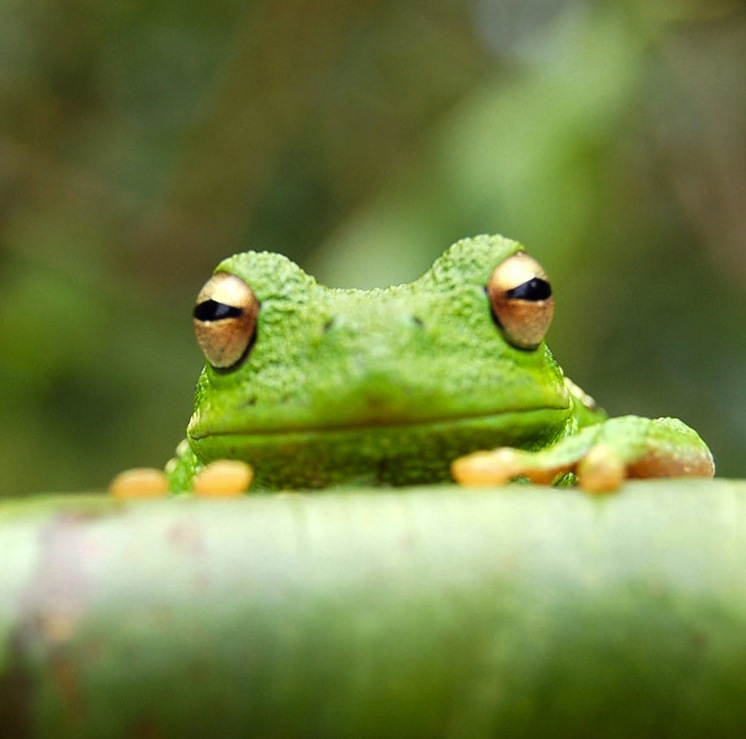
\includegraphics[width=0.3\textwidth]{frog.jpg}
%\caption{\label{fig:frog}This is a frog - i like frogs}
%\end{figure}






\section{Conclusion}

Conclusion


\newpage

\bibliography{bibliography.bib}

\end{document}